% il tipo article
\documentclass[a4paper]{article}
\usepackage[main=english,italian]{babel}
%\usepackage{Times}
%\usepackage[utf8]{inputenc}
\usepackage[hidelinks]{hyperref}%con la package hyperref normale si vedono delle linee rosse nella parte di Contents e References.
\usepackage{xcolor}

\usepackage{graphicx} %  imagini

\definecolor{ao}{rgb}{0.0, 0.0, 1.0}
\newcommand{\ao}[1]{{\color{ao}[#1]}}




\title{Video Stabilization}
\author{Ledjo Lleshaj  VR450678}
%\author{III anno Informatica triennale}
\date{III anno Informatica triennale}
\begin{document} 
	\maketitle 
	
	\newpage % nuova pagina
	\tableofcontents % index // indice
	
	\newpage 
	\section{Video Stabilization Using Point Feature Matching} 
	
 One way to stabilize a video is to track a salient feature in the image and use this as an anchor point to cancel out all perturbations relative to it. This procedure, however, must be bootstrapped with knowledge of where such a salient feature lies in the first video frame. In this example, we explore a method of video stabilization that works without any such a priori knowledge. It instead automatically searches for the "background plane" in a video sequence, and uses its observed distortion to correct for camera motion.

This stabilization algorithm involves two steps. First, we determine the affine image transformations between all local frames of a video sequence using the estimateGeometricTransform2D function applied to point correspondences between two images. Second, we warp the video frames to achieve a stabilized video. We will use the Computer Vision Toolbox™, both for the algorithm and for display.
	\subsection{Feature Detection}
	Our goal is to determine a transformation that will correct for the distortion between the two frames. We can use the estimateGeometricTransform2D function for this, which will return an affine transform. As input we must provide this function with a set of point correspondences between the two frames. To generate these correspondences, we first collect points of interest from both frames, then select likely correspondences between them.
	%\hfill \break
		
	\begin{figure}[htpb!] 
		\centering 
		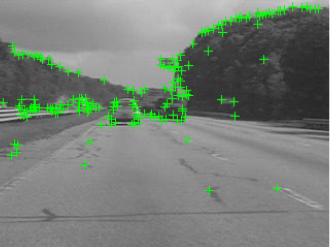
\includegraphics{FeatureDetection.png}
	\end{figure}
	The detected points from the frame are shown in the figure.
	\hfill \break
	In this step we produce these candidate points for each frame. To have the best chance that these points will have corresponding points in the other frame, we want points around salient image features such as corners. For this we use the detectFASTFeatures function, which implements one of the fastest corner detection algorithms.
	
	\subsection{Feature Matching}
	Next we pick correspondences between the points derived above.Many of the point correspondences obtained in the previous step are incorrect. But we can still derive a robust estimate of the geometric transform between the two images using the M-estimator SAmple Consensus (MSAC) algorithm, which is a variant of the RANSAC algorithm. The MSAC algorithm is implemented in the estimateGeometricTransform2D function. This function, when given a set of point correspondences, will search for the valid inlier correspondences. From these it will then derive the affine transform that makes the inliers from the first set of points match most closely with the inliers from the second set. 
	A limitation of the affine transform is that it can only alter the imaging plane. Thus it is ill-suited to finding the general distortion between two frames taken of a 3-D scene, such as with this video taken from a moving car. But it does work under certain conditions that we shall describe shortly.
	Below is a color composite showing frame A overlaid with the reprojected frame B, along with the reprojected point correspondences. The results are excellent, with the inlier correspondences nearly exactly coincident. The cores of the images are both well aligned, such that the red-cyan color composite becomes almost purely black-and-white in that region.
	
	Note how the inlier correspondences are all in the background of the image, not in the foreground, which itself is not aligned. This is because the background features are distant enough that they behave as if they were on an infinitely distant plane. Thus, even though the affine transform is limited to altering only the imaging plane, here that is sufficient to align the background planes of both images. Furthermore, if we assume that the background plane has not moved or changed significantly between frames, then this transform is actually capturing the camera motion. Therefore correcting for this will stabilize the video. This condition will hold as long as the motion of the camera between frames is small enough, or, conversely, if the video frame rate is high enough.
	\begin{figure}[htpb!] 
		\centering 
		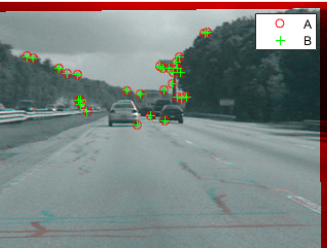
\includegraphics{FeatureMatching.png}
	\end{figure}
	The best points from feature matching are shown in the figure.
	\hfill \break
	\subsection{Offset reverting,smoothing and anti-transforming the changes}
	Now we apply the above steps to smooth a video sequence. For readability, the above procedure of estimating the transform between two images has been placed in the MATLAB function cvexEstStabilizationTform. The function cvexTformToSRT also converts a general affine transform into a scale-rotation-translation transform.
	
	At each step we calculate the transform H between the present frames. We fit this as an s-R-t transform, HsRt. Then we combine this the cumulative transform, Hcumulative, which describes all camera motion since the first frame. The last two frames of the smoothed video are shown in a Video Player as a red-cyan composite.
	\section{Video stabilization using anchor of our choice}
	
	\subsection{Frame rotating according to the offset calculated with Fourier}
	Since the amplitude spectrum of an image is invariant with respect to the translation then we can start thinking about doing the rotation before the traslation. The idea then is to calculate the Fourier transform of the first frame and save it. For each next frame then, we calculate the Fourier transform and rotate it with a series of different angles and for each of these we calculate the cross-correlation coefficient. We use the angle that produces the  max coefficient to rotate the frame in the space domain and obtain the correct image with respect to the rotation.
	
	\begin{figure}[htpb!] 
		\centering 
		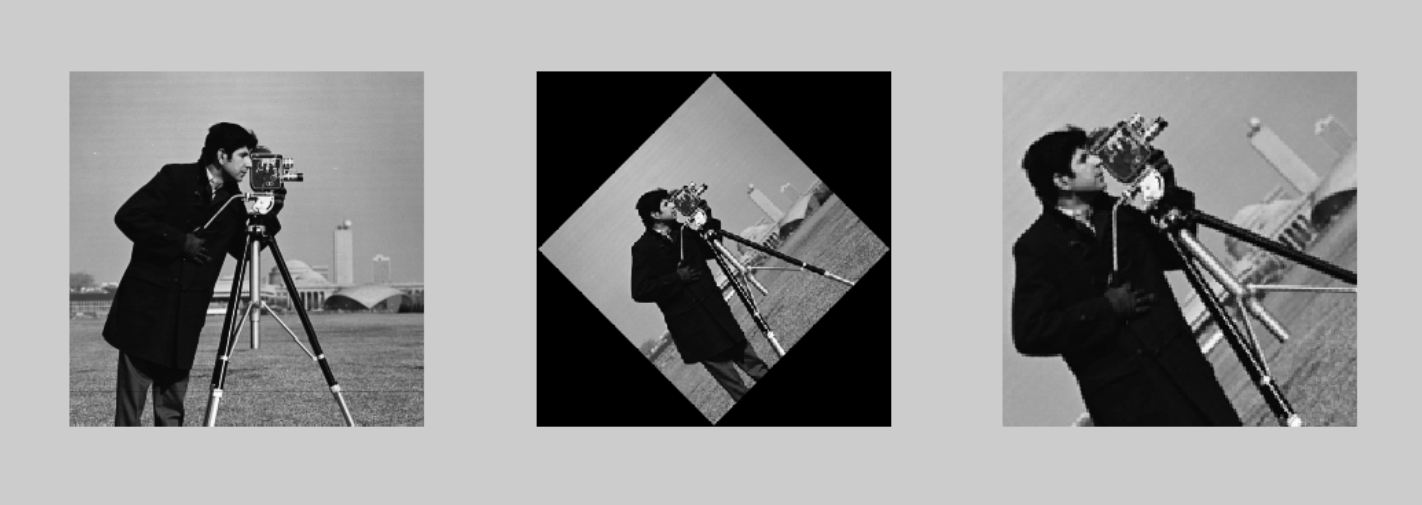
\includegraphics[width=100mm]{ImageRotation.png}
	\end{figure}
	Example of an Image rotated

	\subsubsection{Different dimensions problem}
	The problem now is that the frames are corrected with respect to the rotation of the entire image. Instead we want that stabilization aims to stabilize the template only.so that's why we use the cross-correlation coefficient between the transform of the frame and the transform of the template (instead of the of the entire first frame).
	The template and the frames do not have the same dimension, so the same goes for their transforms. As a result, the cross-correlation coefficient between the latter.	What I do to solve this problem is a zero-padding of the template, before the calculation of the	transformed, so as to bring it to have the same resolution as the video.
	\subsubsection{Calculating the Zero Padding vector}
	If we apply this rotation to the frame without cropping we risk altering the size of the frame, the which is not desirable.If instead we use cropping, we cut away the corners of the image that end up outside the painting. But there is the possibility that the correction with respect to the translation brings back those portions of the image in view. We should therefore rotate the frame but, somehow, preserve it entirely.To do this, I wrote a function that takes an image as input and returns the quantities of which do zero-padding on the vertical and horizontal axis to allow rotation with crop without loss of	information.
	This function is performed on the first frame and the result is saved in a variable so that it can be later used with the standard library padarray function.The padding operation is performed on the frames before being rotated. Following the padding we have to calculate the offset and correct the translation. As the images are now larger in size, too must be calculated on the first frame after the same padding has been applied to it.
	\subsubsection{Cropping}
	Now that we have applied all the transformations, all that remains is to remove the padding previously applied and return the frame to its original size, discarding the information at the edges.
	
	\subsection{Frame Traslation}
	\begin{figure}[htpb!] 
		\centering 
		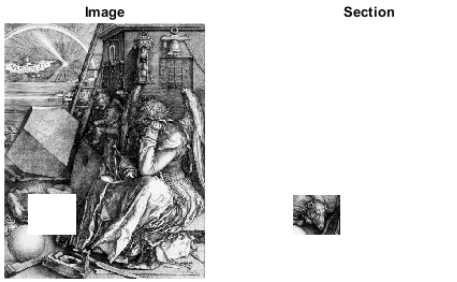
\includegraphics[height=50mm]{ImageTraslation.png}
	\end{figure}
	%\hfill \break
	Frame traslating can be easily done by calculating the offset and then running a 2D cross-correlation on every frame.I have implemented a findoffset function that takes an image and a template as input and returns the vector with the coordinates that the upper left corner of the template must have to be correctly traslated on the image.
	To do this, the function converts the image from RGB to grayscale (if 3 dimension image RGB), performs the 2D cross correlation, finds the maximum point and subtracts the dimensions of the template.
	Howerver the frames following the first frame are translated in order to bring the template back to the same position in which it was in the first frame, and not in the center of the picture frame. To do this, I run the findoffset function with the first frame and save in an variable the
	result. For all subsequent frames I run findoffset and subtract the initial offsset from the result. This indicates the shift that the template has made within the image from the first frame to that considered.In order to revert the changes the template has made we need to use the opposite vector of the one found with the subtraction .This way the corresponding portion of the image the template should go back to where it was.

	\newpage
	
	% Bibliografia. 
	%\subsection{Bibliografia}
	\begin{thebibliography}{10}
		\item \href{https://it.mathworks.com/help/vision/ug/video-stabilization-using-point-feature-matching.html#videostabilize_pm-6/}{\ao{Point Feature Matching}}
		\item 
		\href{https://homepages.inf.ed.ac.uk/rbf/HIPR2/fourier.htm}{\ao{Fourier Transform on image processing}}
		\item 
		\href{https://it.mathworks.com/help/images/fourier-transform.html}{\ao{Fourier Transform on image processing}}
		\item 
		\href{https://www.researchgate.net/publication/4156296_Full-frame_video_stabilization}{\ao{Full-frame video stabilization}}
		
	\end{thebibliography}
	
\end{document}
